\documentclass{beamer} %[12pt]
\usepackage{xcolor}
%\usetheme{boadilla}
%\usetheme{malmoe}
%\usetheme{copenhagen}
%\usecolortheme{rose}
\usecolortheme{beaver}
\usepackage{pgf, graphics}
\usepackage{graphicx}
%\usepackage[left=3cm,top=3cm,right=3cm,nohead,nofoot]{geometry}
\usepackage{hyperref}
\usepackage{setspace}
\usepackage[square]{natbib}
\usepackage{amsmath}
\usepackage{amssymb}
\usepackage{verbatim}
\usepackage{color}
\usepackage{fancyvrb}
\usepackage{bbm}

\begin{filecontents}{ref.bib}
\end{filecontents}

%\usetheme{EastLansing}
%\usepackage{natbib}
\bibliographystyle{apalike}
% make bibliography entries smaller
%\renewcommand\bibfont{\scriptsize}
% If you have more than one page of references, you want to tell beamer
% to put the continuation section label from the second slide onwards
\setbeamertemplate{frametitle continuation}[from second]
% Now get rid of all the colours
\setbeamercolor*{bibliography entry title}{fg=black}
\setbeamercolor*{bibliography entry author}{fg=black}
\setbeamercolor*{bibliography entry location}{fg=black}
\setbeamercolor*{bibliography entry note}{fg=black}
% and kill the abominable icon
\setbeamertemplate{bibliography item}{}


\newcommand{\hl}[1]{\colorbox{yellow}{#1}}
\newcommand{\hlblue}[1]{\colorbox{green}{#1}}
\newcommand{\hlblu}[1]{\colorbox{cyan}{#1}}
\newcommand{\hlred}[1]{\colorbox{cyan}{#1}}
\newcommand{\hlre}[1]{\colorbox{pink}{#1}}
\newcommand{\hlgreen}[1]{\colorbox{pink}{#1}}
\newcommand{\hlgree}[1]{\colorbox{green}{#1}}



\DeclareMathOperator*{\argmax}{\arg\!\max}

\DeclareMathOperator*{\argmin}{\arg\!\min}


\newcommand{\specialcell}[2][c]{%
  \begin{tabular}[#1]{@{}c@{}}#2\end{tabular}}



%\setbeamersize{text margin left=.5cm,text margin right=.5cm}
\newenvironment{changemargin}[2]{%
  \begin{list}{}{%
    \setlength{\topsep}{0pt}%
    \setlength{\leftmargin}{#1}%
    \setlength{\rightmargin}{#2}%
    \setlength{\listparindent}{\parindent}%
    \setlength{\itemindent}{\parindent}%
    \setlength{\parsep}{\parskip}%
  }%
  \item[]}{\end{list}}
\setbeamertemplate{navigation symbols}{}%remove navigation symbols
\usepackage{color}
\newcommand{\hilight}[1]{\colorbox{yellow}{#1}}
\setbeamertemplate{footline}[page number]

\begin{document}


\title[dedup]{Today:  Networks}


\author[Samuel L. Ventura]{\\
  \large{Sam Ventura\\36-315\\Today:  Networks}}
\institute[CMU Statistics]{Department of Statistics\\Carnegie Mellon University}
\date{\today}


\begin{frame}
	\maketitle

	
\end{frame}



\begin{frame}\frametitle{Networks}
	\small
	
	\textbf{Examples of networks:}
	
	\vskip 2 cm
	
	\textbf{Basic Network Structure:}
	
	\vskip 10 cm
	
\end{frame}




\begin{frame}\frametitle{Adjacency Matrices}
	\small
	
	\textbf{Adjacency Matrix}:  representation of the network in matrix form
	
	\vskip 4 cm
	
	\vskip 10 cm
	
\end{frame}




\begin{frame}\frametitle{Visualizing Networks}
	\small
	
	\textbf{Layout}:  Trying to position the nodes to ``maximize'' visualization corresponding to specific criteria
	
	\vskip 4 cm
	
	
	\vskip 10 cm
	
\end{frame}




\begin{frame}\frametitle{Oral Evaluation Graphic -- ``Radar Chart''}
	\small
	\centering
	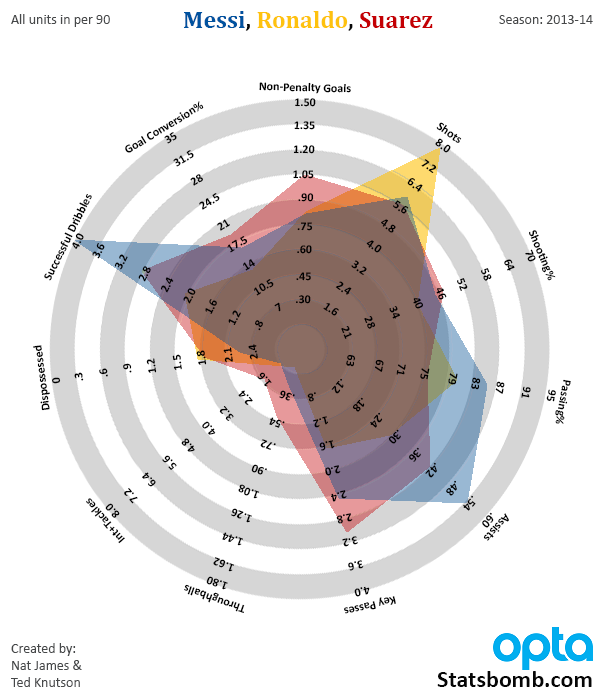
\includegraphics[width = 0.66\linewidth]{radar.png}
	
\end{frame}



\begin{frame}\frametitle{Radar Charts and Parallel Coordinates}
	\small
	\textbf{Radar Charts:}
	
	\vskip 4 cm
	
	\textbf{Parallel Coordinates:}
	
	\vskip 10 cm
	
\end{frame}


\end{document}
